\documentclass[12pt]{article}

\usepackage{amsmath}
\usepackage{amssymb}
\usepackage{amsthm}
\usepackage{hyperref}
\usepackage[pdftex]{graphicx}
%\usepackage{physymb}
%\usepackage{wrapfig}
\usepackage{braket}
\usepackage{subcaption}
\title{PH 304: Assignment 2}

\author{Manish Goregaokar (120260006)}
\date{January 26, 2015}
\begin{document}
\maketitle
\section*{Problem 1}

$$n! = \int_0^\infty e^{-x}x^n dx$$

Integrating by parts,
\begin{align*}
I_n &= \left.x^n\int e^{-x}\right|_0^\infty + \int_0^\infty nx^{n-1}\int e^{-x}\\
 &= - \left.x^n e^{-x}\right|_0^\infty + nI_{n-1}\\
 &= nI_{n-1}\\
 \therefore I_n &= nI_{n-1}
\end{align*}

Additionally, for $n=0$, $I_0 = \int_0^\infty e^{-x} = 1$. So $I_0 = 1,  I_n = nI_{n-1}$. From this we see that this is exactly the factorial function, which obeys the same recursion relation.$\hfill$ Ans. (i)

\begin{figure}[!htb]
\centering
\begin{subfigure}[b]{0.4\textwidth}
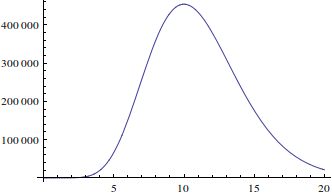
\includegraphics[scale=0.5]{gamma10}
\caption{Integrand for $n=10$}
\end{subfigure}
~~~
\begin{subfigure}[b]{0.4\textwidth}
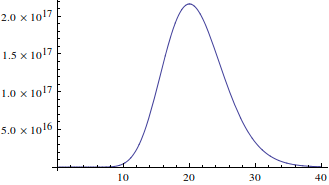
\includegraphics[scale=0.5]{gamma20}
\caption{Integrand for $n=20$}
\end{subfigure}
\\~\\~
\begin{subfigure}[b]{0.4\textwidth}
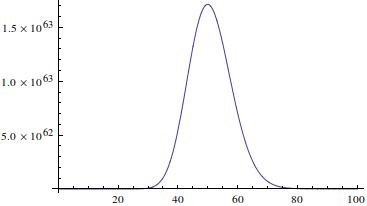
\includegraphics[scale=0.5]{gamma50}
\caption{Integrand for $n=50$}
\end{subfigure}
\end{figure}

$$g(x)=A\exp\left(-\frac{(x-x_0)^2}{2\sigma^2}\right)$$

Now, $g(x) \approx e^{-x}x^n$. We take the Taylor expansion about the maxima $x=x_0$.
 \begin{align*}
e^{-x}x^n &=x_0^n e^{-x_0} + 0 +
\frac{(x-x_0)^2}{2}\left.\frac{d^2}{dx^2}e^{-x  +n\ln x}\right|_{x=x_0} + \dots\\
&=x_0^n e^{-x_0} + 0 +\frac{(x-x_0)^2}{2}\left(e^{-x_0} x_0^{n-2} \left(-2 n x_0+(n-1) n+x_0^2\right)\right)
\end{align*}

Whereas for the Gaussian, the Taylor expansion about the mean is $A(1 + 0(x-x_0) - \frac{(x-x_0)^2}{2}\frac{1}{ \sigma ^2}$

Thus, $A = x_0^ne^{-x_0}$, $-\frac{1}{ \sigma ^2} = 1 - \frac{2n}{x_0} + \frac{n(n-1)}{x_0^2}$


To find $x_0$, we set the derivative to zero: $n e^{-x} x^{n-1}-e^{-x} x^n = 0$, and we find that $x_0 = n$

Thus, $\boxed{A=n^ne^{-n}}$, $\boxed{x_0 = n}$, $\frac{1}{\sigma^2} = 1-\frac{n-1}{n}$, and $\boxed{\sigma = \sqrt{n}}$

While the higher deriviatives of these two functions diverge for large $n$, the approximation still comes closer when plotted. Thus, this approximation improves as $n$ becomes large, but the two curves are not asymptotically equal.

\begin{figure}[!htb]
\centering
\begin{subfigure}[b]{0.4\textwidth}
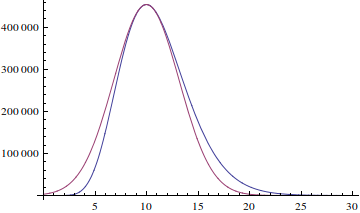
\includegraphics[scale=0.5]{gaus10}
\caption{Gaussian approximation  for $n=10$}
\end{subfigure}
~~~
\begin{subfigure}[b]{0.4\textwidth}
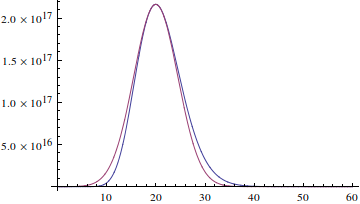
\includegraphics[scale=0.5]{gaus20}
\caption{Gaussian approximation  for $n=20$}
\end{subfigure}
\\~\\~
\begin{subfigure}[b]{0.4\textwidth}
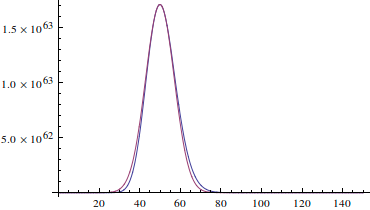
\includegraphics[scale=0.5]{gaus50}
\caption{Gaussian approximation for $n=50$}
\end{subfigure}
\end{figure}
\begin{figure}[!htb]
\centering
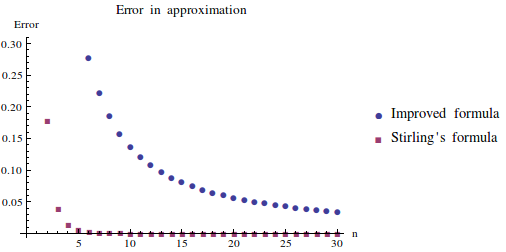
\includegraphics[scale=0.5]{error}
\end{figure}
\newpage
\section*{Problem 2}

Let us take the random variable $y = \left\lbrace\begin{array}{ll}1 & \text{if} (x-\lambda)^2 > k^2\\
0 & \text{if} (x-\lambda)^2 \leq k^2\end{array}\right.$

$\therefore E(y) = P(\text{x is not in $k$ neighborhood})$

Additionally, if $x >0$, $y \leq \frac{(x-\lambda)^2}{k^2}$. Thus, $E[y] \leq E[\frac{(x-\lambda)^2}{k^2}] ~\implies~ P(\text{x is not in } k \text{ neighborhood}) \leq \frac{\sigma^2}{k^2}$

If $n\sigma = k$, we get $\boxed{P(\text{x is not in } n\sigma \text{ neighborhood}) \leq \frac1{n^2}}$

\section*{Problem 3}
\newcommand{\inint}{\int_{-\infty}^\infty}
$$S(\alpha, \beta, p(x)) = -\inint p(x)\ln p(x)dx + \alpha\left(1-\inint p(x)dx\right)+ \beta\left(f-\inint F(x)p(x)dx\right)$$

By lagrange multipliers, \begin{align*}
0 &= -\frac{\delta}{\delta p(y)}\inint p(x)\ln p(x)dx + \frac{\delta}{\delta p(y)} \alpha\left(1-\inint p(x)dx\right)+\frac{\delta}{\delta p(y)}\beta\left(f-\inint F(x)p(x)dx\right)\\
&= -\inint \ln p(x)\delta(x-y) - \inint \delta{x-y} - \alpha\inint \delta{x-y} -F(x)\beta\inint \delta{x-y} \\
&= -(1+\ln p(y)) - \alpha - F(x)\beta
\end{align*} 
Thus, $p(y) = \exp(-1-\alpha - \beta F(x))$
When $\Braket{|v|} = c$, we have the equations:
\begin{align*}
p(x) &= \exp(-1-\alpha - \beta |x|)\\
\inint p(x) dx &= 1\\
\inint |x| p(x) dx &= c\\
\therefore 1 &= \inint \exp(-1-\alpha - \beta |x|) \\
 &= 2\int_0^\infty \exp(-1-\alpha - \beta x)\\
 &= \frac{2}{\beta}e^{-1-\alpha}\\
 \therefore p(y) &= \frac{\beta}{2} e^{-\beta|x|}\\
 \text {Now, } \inint |x| p(x) dx &= c\\
 \therefore c &= 2\int_0^\infty x\frac{\beta}{2} e^{-\beta x}dx \\
 c &= \frac{1}{\beta}\\
 \beta &= \frac1 c
\end{align*}

Thus, for constraining $\Braket{|v|} = c$, the distribution is $\boxed{p(v) = \frac1{2c} e^{-\frac{1} {c}v}}\hfill$ Ans.

When constraining $\Braket{v^2} = c^2$, we have 
\begin{align*}
p(x) &= \exp(-1-\alpha - \beta x^2)\\
\inint p(x) dx &= 1\\
\inint |x| p(x) dx &= c\\
\therefore 1 &= \inint \exp(-1-\alpha - \beta x^2) \\
 &= 2\int_0^\infty \exp(-1-\alpha - \beta x^2)\\
 &= e^{-1-\alpha}\sqrt{\frac{\pi}{\beta}}\\
 \therefore p(y) &= \sqrt{\frac{\beta}{\pi}} e^{-\beta x^2}\\
 \text {Now, } \inint x^2 p(x) dx &= c\\
 \therefore c &= 2\int_0^\infty x^2 2 e^{-\beta x^2}dx \\
 c &=  2 \sqrt{\frac{\beta}{\pi}}\frac{\sqrt{\pi}}{4 \beta^{3/2}}\\
 \beta &=\frac{1}{2 c}
 \end{align*}
 
 Thus, for constraining $\Braket{v^2} = c^2$, the distribution is $\boxed{p(v) = \sqrt{\frac{\beta}{\pi}} e^{-\frac{1} {2c}v^2}}\hfill$ Ans.
\section*{Problem 4}
This is a binomial distribution.

The mean of one question will be $7$, with standard deviation $\sqrt{0.7(1-0.3)} = 0.458258$. For the exam, the mean will be $70$ with standard deviation $\sqrt{10\times 0.7(1-0.3)} = 1.44914$

\section*{Problem 5}

Here, RMS distance should be R. Thus, $\sqrt{\Braket{x_N^2}} = \sqrt{N}l = R \implies N = 5\times 10^{21}$. Thus, it takes approximately $\boxed{5\times 10^{21}}$ steps to reach the radius where convection becomes important.

The time taken will be $5\times 10^{21}\times \frac{l}{c} = \boxed{2.30504\times 10^9 ~\mathrm s}$

\section*{Problem 6}

\begin{figure}[!htb]
\centering
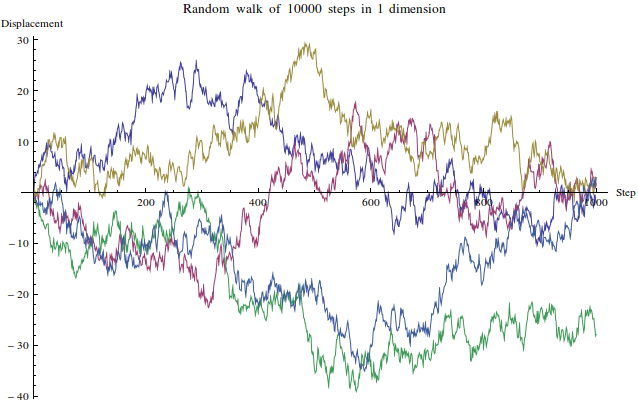
\includegraphics[scale=0.5]{random1}
\end{figure}

\begin{figure}[!htb]
\centering
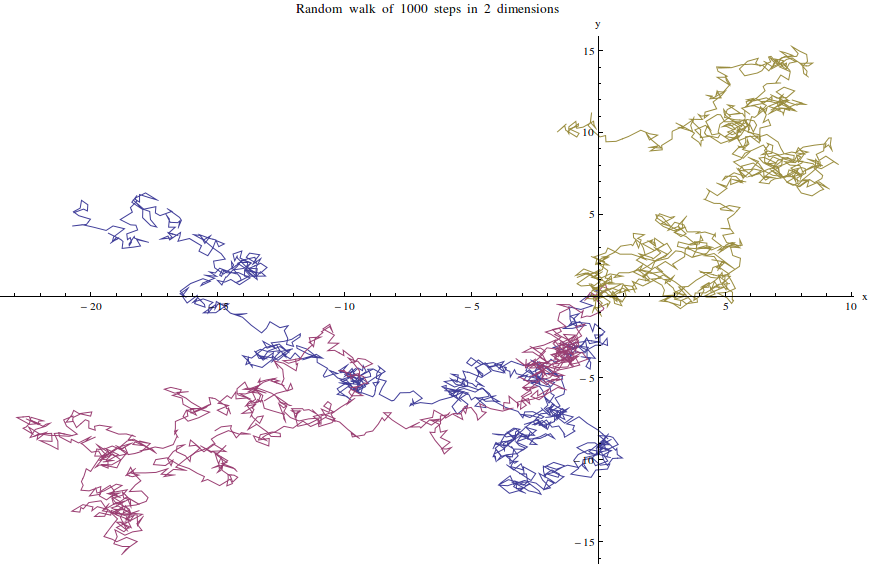
\includegraphics[scale=0.5]{random2sm}
\end{figure}

\begin{figure}[!htb]
\centering
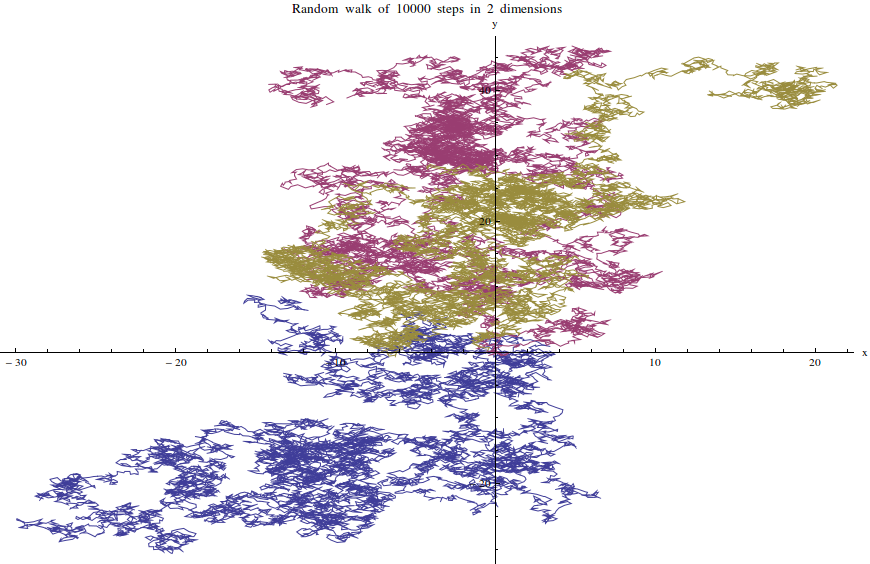
\includegraphics[scale=0.5]{random2lg}
\end{figure}
\begin{figure}[!htb]
\centering
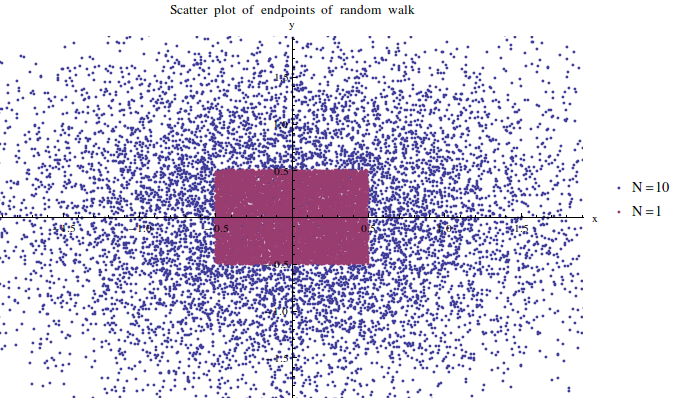
\includegraphics[scale=0.5]{scatter}
\end{figure}

Such a variable has a density function as $f(x) = 1$ for all $x$ in the region $[-0.5, 0.5]$. Its RMS step size will be $\sqrt{\int_{-0.5}^{0.5}x^2=\frac1{12}}$, giving us $\boxed{\frac1{2\sqrt3}}$.

\begin{figure}[!htb]
\centering
\begin{subfigure}[b]{0.4\textwidth}
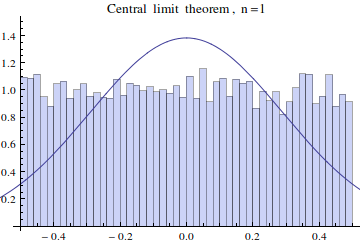
\includegraphics[scale=0.4]{central1}
\end{subfigure}
~~~
\begin{subfigure}[b]{0.4\textwidth}
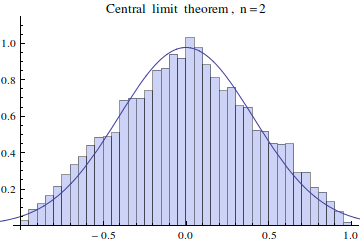
\includegraphics[scale=0.4]{central2}
\end{subfigure}
\\~\\~
\begin{subfigure}[b]{0.4\textwidth}
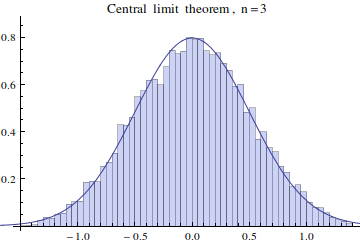
\includegraphics[scale=0.4]{central3}
\end{subfigure}
~~~
\begin{subfigure}[b]{0.4\textwidth}
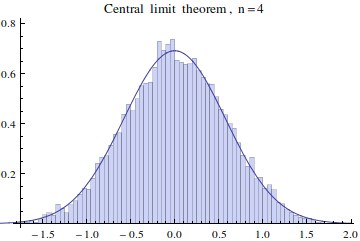
\includegraphics[scale=0.4]{central4}
\end{subfigure}
\\~\\~
\begin{subfigure}[b]{0.4\textwidth}
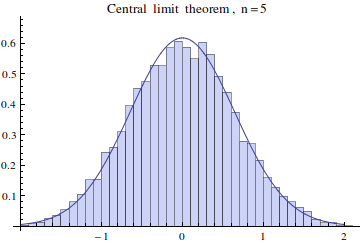
\includegraphics[scale=0.5]{central5}
\end{subfigure}
\caption{As seen in the graphs above, the Gaussian approximates the random walk very quickly.}
\end{figure}


\end{document}
